\documentclass[tikz,border=3.14mm]{standalone}
\usepackage{pgfplots}

\begin{document}
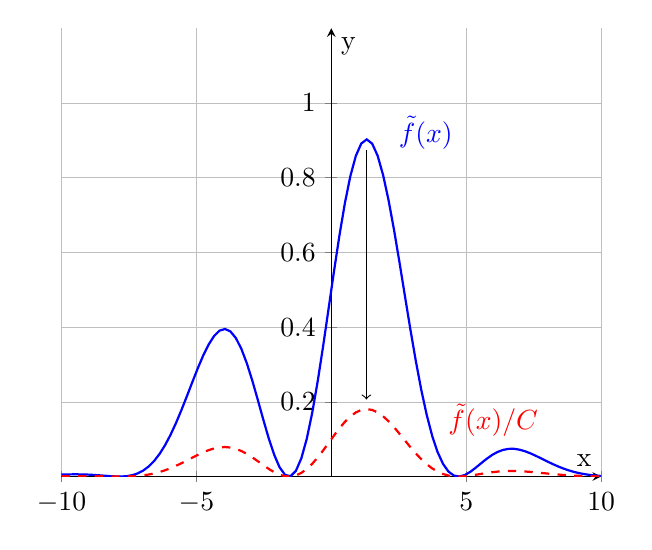
\begin{tikzpicture}
\begin{axis}[
    xlabel={x},
    ylabel={y},
    xmin=-10, xmax=10,
    ymin=0, ymax=1.2,
    xtick={-10,-5,0,5,10},
    ytick={0,0.2,0.4,0.6,0.8,1},
    grid=both,
    grid style={line width=.1pt, draw=gray!10},
    major grid style={line width=.2pt,draw=gray!50},
    axis lines=middle,
    samples=100,
]

% Original wiggly non-negative function (like sin(x) convolved with a wide normal distribution)
\addplot[blue, thick, domain=-10:10] {0.5*exp(-x^2/20)*(sin(deg(x)) + 1)};
% Normalized function (integral equals 1), dashed line
\addplot[red, dashed, thick, domain=-10:10] {0.1*exp(-x^2/20)*(sin(deg(x)) + 1)};

\node (source) at (axis cs:1.3, .9) {};
\node (destination) at (axis cs:1.3, .18) {};
\draw [->] (source) -- (destination);

\node [blue] at (axis cs:3.5, .92) {$\tilde{f}(x)$};
\node [red] at (axis cs:6, .15) {$\tilde{f}(x)/C$};

\end{axis}
\end{tikzpicture}
\end{document}
